\newpage
\subsection{Mounting Solutions}
The selected drone must be able to fit one or more sensors described in  \ref{variables} Variables. One or more add-on(s) for the drone needs to be developed to fit these sensors that passes several requirements:

\begin{itemize}
    \item \textbf{Waterproof}
          \begin{itemize} 
            \item The add-on will be submerged in sea water for an extended period of time. Therefore it is important that the mounting solution doesn't deteriorate in this water. 
          \end{itemize}
    \item \textbf{Swappable}
          \begin{itemize} 
            \item In case of multiple mounting solutions, they need to be able to be easily swapped during the testing site
          \end{itemize}
  \item \textbf{Nondestructive to the drone}
          \begin{itemize} 
            \item In order to not void the warranty or any guarantees of functioning of the drone, the modifications made to it must be nondestructive.
          \end{itemize}
  \item \textbf{Easy to extend and edit}
        \begin{itemize} 
            \item It is useful if the add-on can be easily edited from it's original design in case of an error or additional uses
        \end{itemize}
\end{itemize}

\subsubsection{3D Printing}
Mounts for the sensors can be 3D printed as long as the design is simple to avoid air gaps. The material also should not deteriorate in the water. PET is the preferred filament for creating waterproof prints because of its relative smooth finish and chemical resistance. \cite{pet}

\begin{figure}[h]
\centering
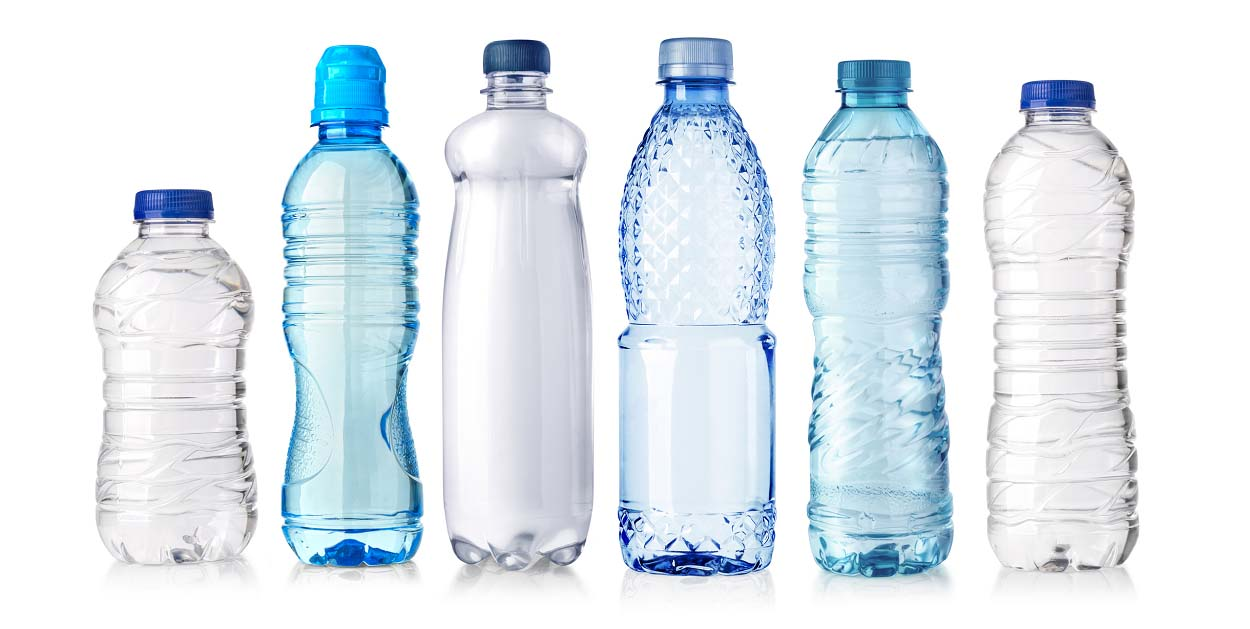
\includegraphics[scale=0.2]{uav/31_pet.jpg}
\caption{PET is commonly used to create water bottles \cite{petbottle}}
\end{figure}

To avoid air gaps, one can purposely over-extrude the prints, though this makes the mount heavier. After printing, one should smooth out the print using acetone, epoxy, or wax \cite{waterproof3d}. 3D printing has the advantage in that the prints are easy to reproduce using a CAD model and print settings. Plastic mounts also tend to be more lightweight and durable than wood or metal when used in aquatic applications. PET has a disadvantage in that it sags a lot during printing. Therefore extra attention must be paid to creating designs which have little overhang.  \cite{overhang}